%!TEX root = ../../msc17-game-book.tex

\phChapterWorksheet{Ghostly Charm}{Main Puzzle 5}

Goolia the Ghost was wondering around the Wayward Tavern yesterday when she saw three witches, Flo, Vi, and Ru, seated around a cauldron with the following cards:

    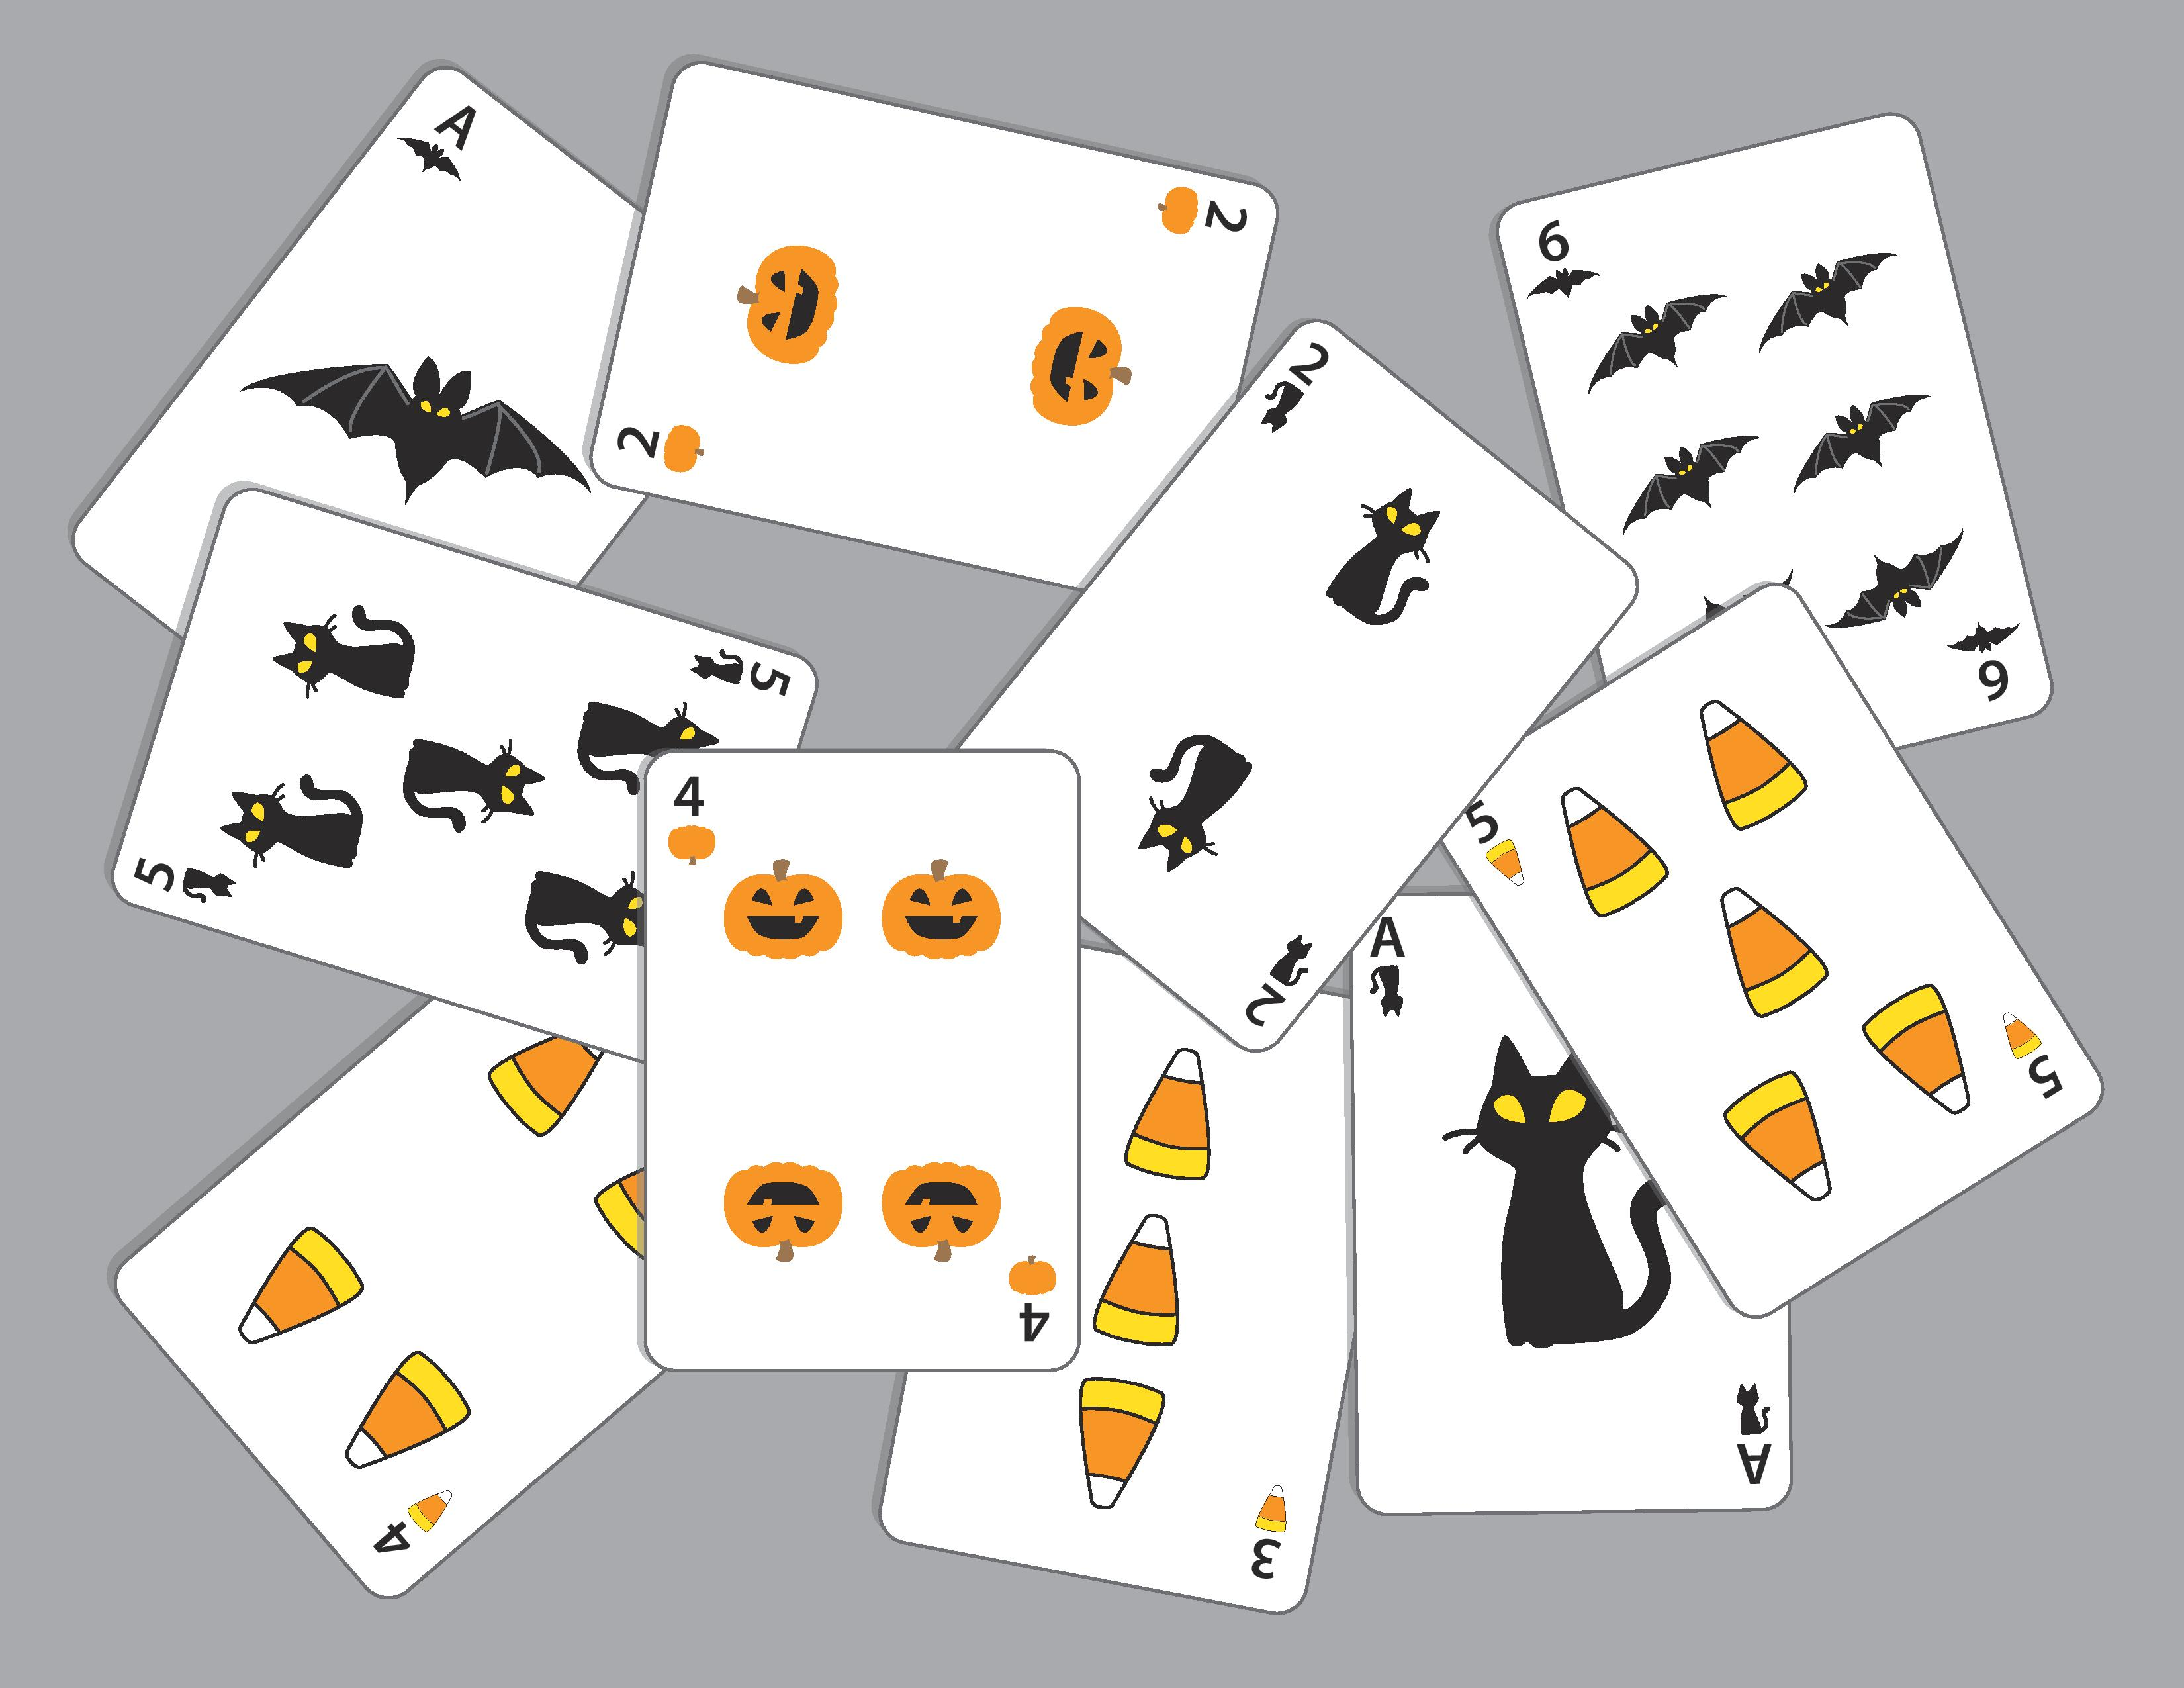
\includegraphics[width=\textwidth]{assets/kat/cardstogeth}

Flo told the other witches that she was going to select one card and give it special powers. She told Vi the suit (Bats, Black Cats, Pumpkins, or Candy Corn) and told Ru the rank (A, 2, 3, 4, 5, or 6). Goolia then heard Vi make the following comment:\\

\textit{Vi: Double double toil and trouble! I don't know what card Flo picked, but I know that Ru doesn't know either!}\\

The witches aren't the only ones interested in knowing what card Flo selected though..\\

\textbf{"Amp'd Squad! I may be a ghost, but I want to know *witch* card has special powers! I know that what Vi said narrows down the possibilities, but I can't quite figure out how! If you can help me figure it out, I'll reward you with a puzzle piece!"}\\


Challenge Overview
\begin{itemize}
\item[*] Follow the logic of the witches' conversation to determine the remaining possibilities of Flo's card.

\item[*] When you think you've got it, go and present your solution to Goolia in \textbf{Challenge Room X}! Make sure you can explain to her how you figured out the answer!
\end{itemize}

\phWorksheet{Cards}

    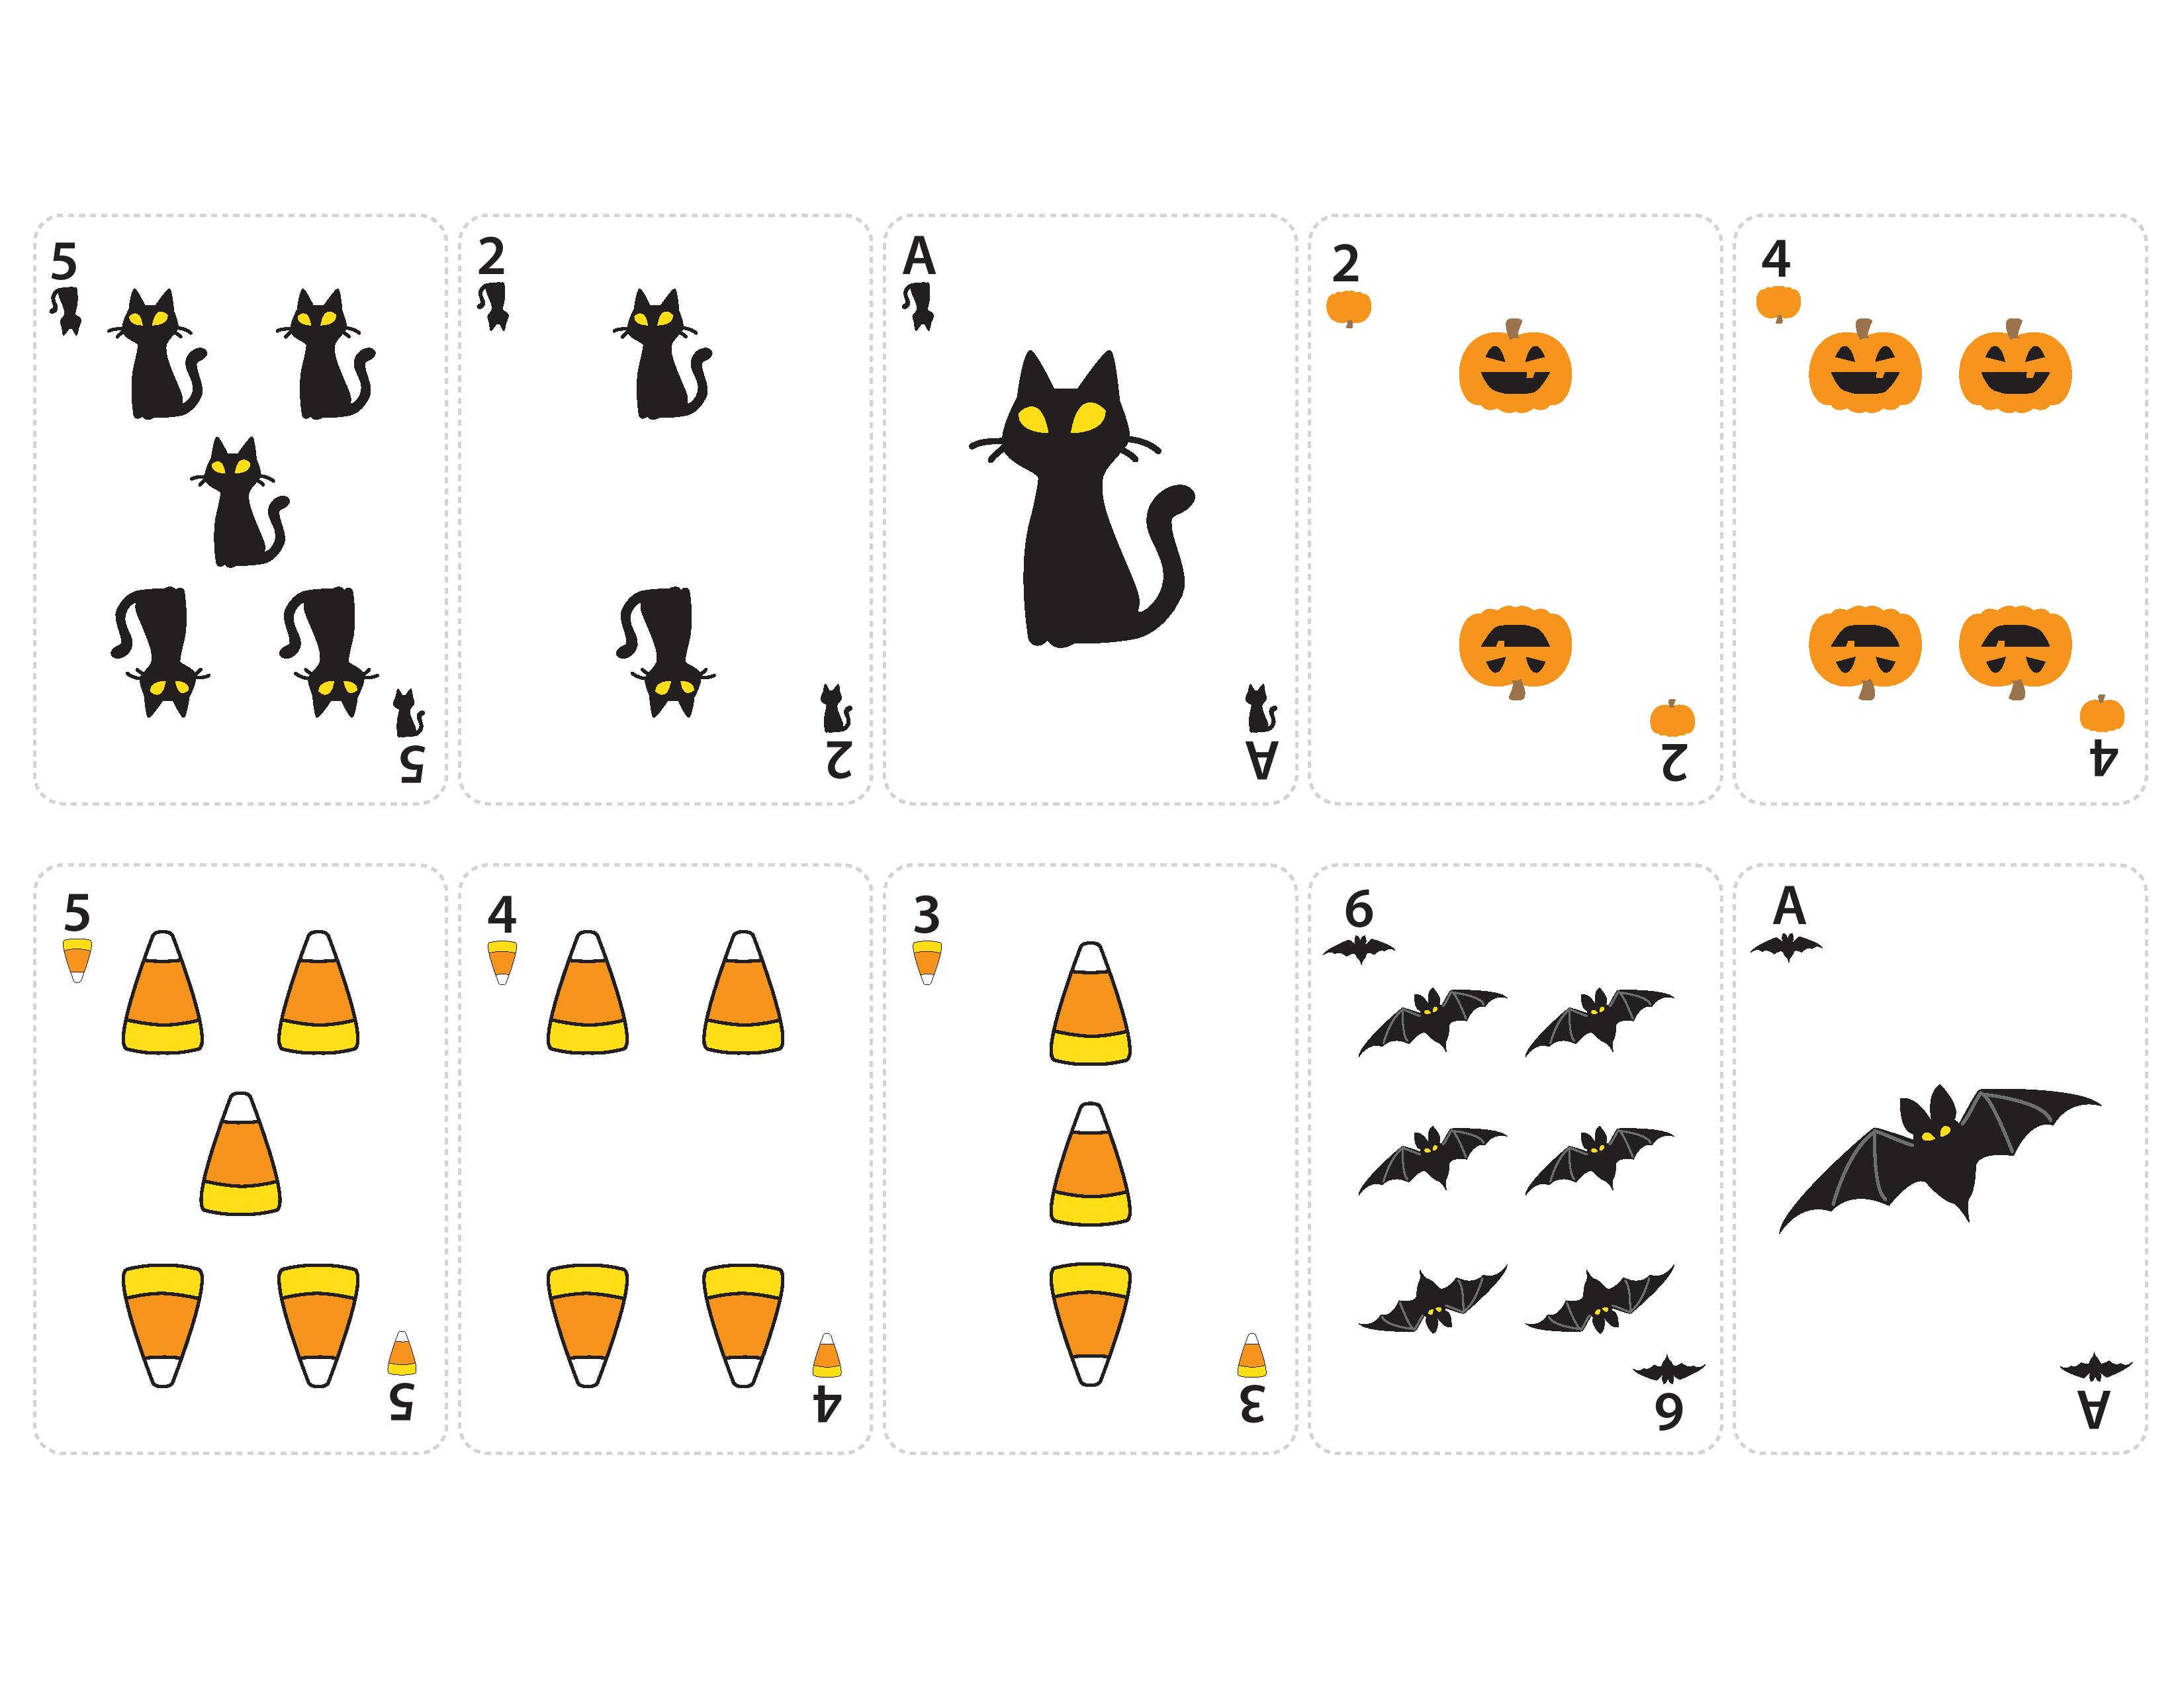
\includegraphics[width=\textwidth,height=\textheight,keepaspectratio, angle =90]{assets/kat/cutouts}
